%----------------------------------------------------------------------------------------
%	2./ INSTRUMENT
%----------------------------------------------------------------------------------------
%\section{General view of the instrument}
%\label{se:instru}

NIKA2 simultaneously images a field-of-view of
6.5' in diameter at 150 and $260\,\rm{GHz}$. It also has polarimetric
capabilities at 260~GHz, which are not discussed here. The optics of
the telescope receiver cabin have been modified in order
to increase the IRAM 30-m telescope field of view. To achieve these
goals without degrading the
telescope angular resolution, NIKA2 employs a total of around
2,900\,KIDs split over three distinct arrays, one for the $150\,\rm{GHz}$
band and two for the $260\,\rm{GHz}$ band.

A detailed description of the instrument can be found in
\citet{Adam2018}. We briefly present here the main sub-systems in this
section focusing on the elements which are specific to NIKA2 or
which drive the development of dedicated procedures for the data reduction or
calibration.


\subsection{Cryogenics}

The optimal operation of the detectors is achieved at a temperature of around
150\,mK, well below the Aluminium superconducting transition. For this reason,
NIKA2 employs a custom dilution fridge to cool down the focal plane, and the
refractive portion of the optics, for a total mass around $100\, \rm{kg}$,
which is kept deeply in the
sub-Kelvin regime. Despite the complexity and huge size of the system, the operation
of NIKA2 does not require external cryogenic liquids and can be fully operated remotely.


\subsection{Optics}

The NIKA2 camera optics include two cold mirrors, and the filtering of
unwanted (off-band) radiation is provided by a suitable stack of
multi-mesh filters placed at all temperature stages between 150 mK and
room temperature. An air-gap dichroic splits the 150\,GHz (reflection)
from the 260\,GHz (transmission) beams. As discussed in
Sect.~\ref{se:flat_field}, the air-gap technology has proven efficient
in preserving the planarity of the dichroic, but shows sub-optimal
performance in tansmission. Moreover, a grid polariser ensures the separation of
the vertical and horizontal components of the linear polarizations
on the 260\,GHz channel. Band-defining filters, custom-designed to
optimally match the atmospheric windows, are installed in
front of each array. A half-wave polarization modulator is added at room
temperature when operating the instrument in polarimetric mode.

Hereafter, the detector array illuminated by the 150\,GHz beam is named Array
2 (A2) from the corresponding observing $2\, \rm{mm}$ waveband,
while in the 260\,GHz ($1\, \rm{mm}$) channel, the array mapping the
horizontal component of the polarization is referred to as Array 1 (A1)
and the one mapping the vertical component is called Array 3 (A3). 

\subsection{KIDs and electronics}
\label{se:array}

Array 2 consists of 616\,KIDs, arranged to cover a 78\,mm diameter
circle. Each camera pixel has a size of
$2.8\times2.8\textrm{\,mm}^2$. Array 2 is connected over four different
readout lines. In the case of the 260\,GHz band detectors, the pixel size is
$2\times 2\mathrm{\,mm}^2$, to ensure a comparable sampling of the focal
plane. In order to fill the two 260\,GHz arrays A1 and A3, a total of
1,140 pixels are needed in each of them. The focal planes are all
based on thin Aluminium films deposited by e-beam evaporation under
ultra-high vacuum conditions over a Silicon substrate.

The key advantage of the KID technology is the simplicity of the cold
electronics and the multiplexing scheme. In NIKA2, each block of around 150
detectors is connected to single coaxial line linked to the readout
electronics~\citep{Bourrion2016}.
%providing the excitation and the
%readout at the two ends. Each of the readout lines is linked to the input of a
%cryogenic (4 K) low-noise amplifier.
The warm electronics required to digitize
and process the pixels signals is composed of twenty custom readout
cards (one per feed-line).

\subsection{KID photometry and {\tt tuning}}
\label{se:tuning}

KIDs are superconducting resonators whose resonance
frequency shifts linearly depending on the incoming optical power. The
measure of such frequency shift $\Delta f$ is critical for the use of
KIDs as mm-wave detectors. 

%For the KID readout, an excitation signal is sent into the cryostat on the
%feedline coupled to the KID.
The excitation tones produced by the
electronics are amplified by a cryogenic (4K) low noise amplifier
before passing through the KIDs and being analysed by the readout
electronics. The transmitted signal can be described by its
amplitude and phase, or, as is common practice for KID, by its Fourier
components that are In-phase ($I$) and in Quadrature $Q$ with respect to the excitation
signal.
The goal is now to relate the measured variations of the KID response
to excitation signal $(\Delta I, \Delta Q)$, which are induced by incident light, to
$\Delta f$. For this, the electronics modulates the excitation
frequency at about 1\,kHz with a known frequency variation $\delta f$
and the read out gives the induced transmitted signal variations
$(dI, dQ)$. Projecting linearly $(\Delta I, \Delta Q)$ on $(dI, dQ)$ therefore
provides $\Delta f$. This quantity, in Hz, constitutes the raw KID
time-ordered data, which are sampled at a frequency of
$23.84\,\rm{Hz}$. For historical reasons, this way of deriving KID
signals has been nicknamed \emph{RfdIdQ}. More details on this process
are given in \citet{Calvo2013}.
%The raw KID data and the telescope pointing data
%are synchronized by the NIKA acquisition system using a clock that
%gives the absolute astrononical time to define the NIKA2 raw data.
Ingested into the calibration pipeline, they will be futher converted
into astronomical units (Sect.~\ref{se:calibration}).\\

In addition to light of astronomical origin, any change in the
background optical load (due, for example, to changes in
the atmospheric emission or in the elevation) contributes as well to
Cooper pair breaking, and thus to the shift of the resonances. In
order to maximize the sensitivity of a KID, the
excitation signal used for the readout must always be near the KID resonance
frequency. We therefore have developped a tuning algorithm that takes care of
this optimization. A {\tt tuning} is performed at the beginning
of each observation scan for the KIDs to be tuned to the background
conditions.
%in order to be optimally set at the same elevation and sky
%conditions as the source.
This process takes only a few seconds
%whenever the resonances are close to the current functionning
%point.
when the frequency shift is small.
These optimal conditions are further maintained by performing
continuous {\tt tunings} between two scans while NIKA2 is not observing, to
adapt regularly with the observing conditions.

\subsection{Bandpasses}
\label{se:instru_bandpass}

\begin{figure}[ht!] % Inline image example
\begin{center}
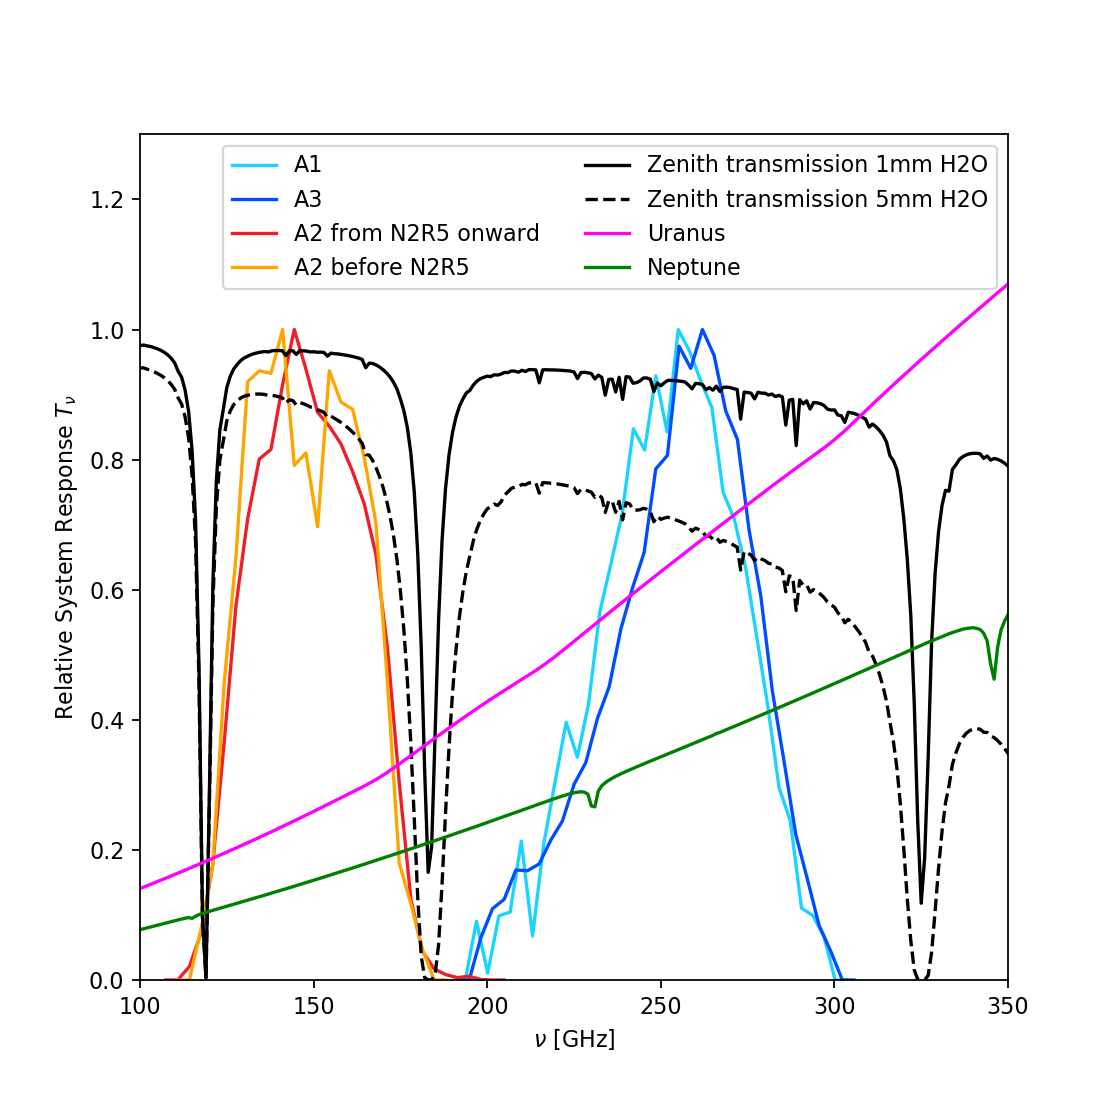
\includegraphics[clip,trim={0, 1cm, 0, 2cm},width=0.5\textwidth]{Figures/bandpasses_nika2_colorsok.png}
\caption[NIKA2 transmission]{Relative system response of the three KID
  arrays as a
  function of frequency. For illustration we also show in black
  the atmospheric transmission obtained with the ATM model \citep{ATM,
    Pardo2002} for two values of precipitable water vapor (1 and
  $5\,\rm{mm}$).
  The spectra of the model of Uranus (pink) and the model of
  Neptune\footnote{These models are available in the Herschel
    Calibrator web page at
    \url{https://www.cosmos.esa.int/web/herschel/calibrator-models}}
  (green) in the frequency range are overplotted with arbitrary
  normalization with respect to the NIKA2 transmission.} 
 \label{spectralband1}
\end{center}
\end{figure}

The NIKA2 spectral bands were measured in the laboratory using a
Martin-Puplett interferometer built in-house~\citep{Durand2007_these}.
The measurement relies on using the difference of two black
body radiations as input signal for the interferometer. 
%Both arrays and filter bands were considered in the measurements. These
%were obtained from the difference of two black bodies, hence they
%include a $\nu^2$ Rayleigh-Jeans (RJ) spectral term.
Figure~\ref{spectralband1} shows the relative spectral response for
the three arrays.  Notice that Array 2 was
upgraded in September 2016 (during the N2R5 technical campaign) and
that the spectral transmissions are slightly different (red and orange lines in
Fig.~\ref{spectralband1}).

The two arrays operating at 260 GHz, mapping different linear polarisations,
exhibit a slightly different spectral behaviour as can be
seen on Fig.~\ref{spectralband1}. This may be explained by a tiny
difference in the silicon wafer and/or Aluminium film
thickness of the KID arrays~\citep{Adam2018}.
%For
%instance, the observed shift of the peak frequency, 265 GHz for the V
%(A1) array versus 258 GHz for the H one (A3), can be explained by
%about 5 microns change in the substrate thickness. 

It is clear from Fig.~\ref{spectralband1} that the atmosphere will
modify the overall transmission of the system, especially at the tails
for A2. In Table~\ref{tab:frequencies}, we give the bandpass-integrated
observing frequencies and bandwidths computed both at zero atmospheric
opacity and for typical winter-semester observing conditions
(defined by an atmospheric content of $2\,\rm{mm}$ of precipitable
water vapor and an observing elevation of $60^o$).

\begin{table}[!htbp]
  \caption[]{Bandpass-integrated observing frequencies and bandwidths
    of the three arrays computed in two different observing conditions}
  \label{tab:frequencies}
  \centering    
  \begin{tabular}{lrrr}
    \hline\hline
    \noalign{\smallskip}
    & Array 1 & Array 3 & Array 2 \\
    \noalign{\smallskip}
    \hline
    \noalign{\smallskip}
    Frequency \small{(0mm, 90deg)} [GHz] & 254.7 & 257.4 &  150.9 \\
    Bandwidth \small{(0mm, 90deg)} [GHz] &  49.2 & 48.0  &   40.7 \\
    Frequency \small{(2mm, 60deg)} [GHz] & 254.2 & 257.1 &  150.6 \\
    Bandwidth \small{(2mm, 60deg)} [GHz] &  48.7 &  47.9 &    39.2 \\
    \noalign{\smallskip}
    \hline
  \end{tabular}
\end{table}
For each array, we define reference frequencies that are chosen
as round numbers in the middle of the bands to define NIKA2
photometric system as will be discussed in
Sect.~\ref{se:calibration}. These are 260~GHz for the A1 and A3 and
150~GHz for A2.
